%%%%%%%%%%%%%%%%%%%%%%%%%%%%%%%%%%%%%%%%%%%%%%%%%%%%%%%%%%%%%%%%%%%%%%
% LaTeX Template: Curriculum Vitae 
% Source: http://www.howtotex.com/
%%%%%%%%%%%%%%%%%%%%%%%%%%%%%%%%%%%%%%%%%%%%%%%%%%%%%%%%%%%%%%%%%%%%%%

\documentclass[paper=a4,fontsize=11pt]{scrartcl} % KOMA-article class
							
\usepackage[english]{babel}
\usepackage{graphicx}                    % Enable pdflatex
\usepackage[svgnames]{xcolor}            % Colors by their 'svgnames'
\usepackage{geometry}
\textheight=650pt
\usepackage{url}
\usepackage{fontawesome}
\usepackage[export]{adjustbox}

\frenchspacing              % Better looking spacings after periods
\pagestyle{empty}           % No pagenumbers/headers/footers

%%% Custom sectioning (sectsty package)
%%% ------------------------------------------------------------
\usepackage{sectsty}

\sectionfont{%			            % Change font of \section command
\usefont{OT1}{phv}{b}{n}%		% bch-b-n: CharterBT-Bold font
\sectionrule{0pt}{0pt}{-5pt}{3pt}}

%%% Macros
%%% ------------------------------------------------------------
\newlength{\spacebox}
\settowidth{\spacebox}{8888888888}			% Box to align text
\newcommand{\sepspace}{\vspace*{1em}}		% Vertical space macro

\newcommand{\MyName}[1]{ % Name
		\Huge \usefont{OT1}{phv}{b}{n} \hfill #1
		\par \normalsize \normalfont}
		
\newcommand{\MySlogan}[1]{ % Slogan (optional)
		\large \usefont{OT1}{phv}{m}{n}\hfill \textit{#1}
		\par \normalsize \normalfont}

\newcommand{\NewPart}[1]{\section*{\uppercase{#1}}}

\newcommand{\PersonalEntry}[2]{
		\noindent\hangindent=0em\hangafter=0 % Indentation
		\parbox{\spacebox}{        % Box to align text
		\textit{#1}}		       % Entry name (birth, address, etc.)
		\hspace{2.5em} #2 \par}    % Entry value

\newcommand{\SkillsEntry}[2]{      % Same as \PersonalEntry
		\noindent\hangindent=0em\hangafter=0 % Indentation
		\parbox{\spacebox}{        % Box to align text
		\textit{#1}}			   % Entry name (birth, address, etc.)
		\hspace{2.5em} #2 \par}    % Entry value	

\newcommand{\EducationEntry}[4]{
		\noindent \textbf{#1} \hfill      % Study
		\colorbox{Black}{%
			\parbox{6em}{%
			\hfill\color{White}#2}} \par  % Duration
		\noindent \textit{#3} \par        % School
		\noindent\hangindent=2em\hangafter=0 \small #4 % Description
		\normalsize \par}

\newcommand{\WorkEntry}[4]{				  % Same as \EducationEntry
		\noindent \textbf{#1} \hfill      % Jobname
		\colorbox{Black}{\color{White}#2} \par  % Duration
		\noindent \textit{#3} \par              % Company
		\noindent\hangindent=2em\hangafter=0 \small #4 % Description
		\normalsize \par}

%%% ------------------------------------------------------------
\begin{document}

\begin{figure}
    \vspace*{60pt}
    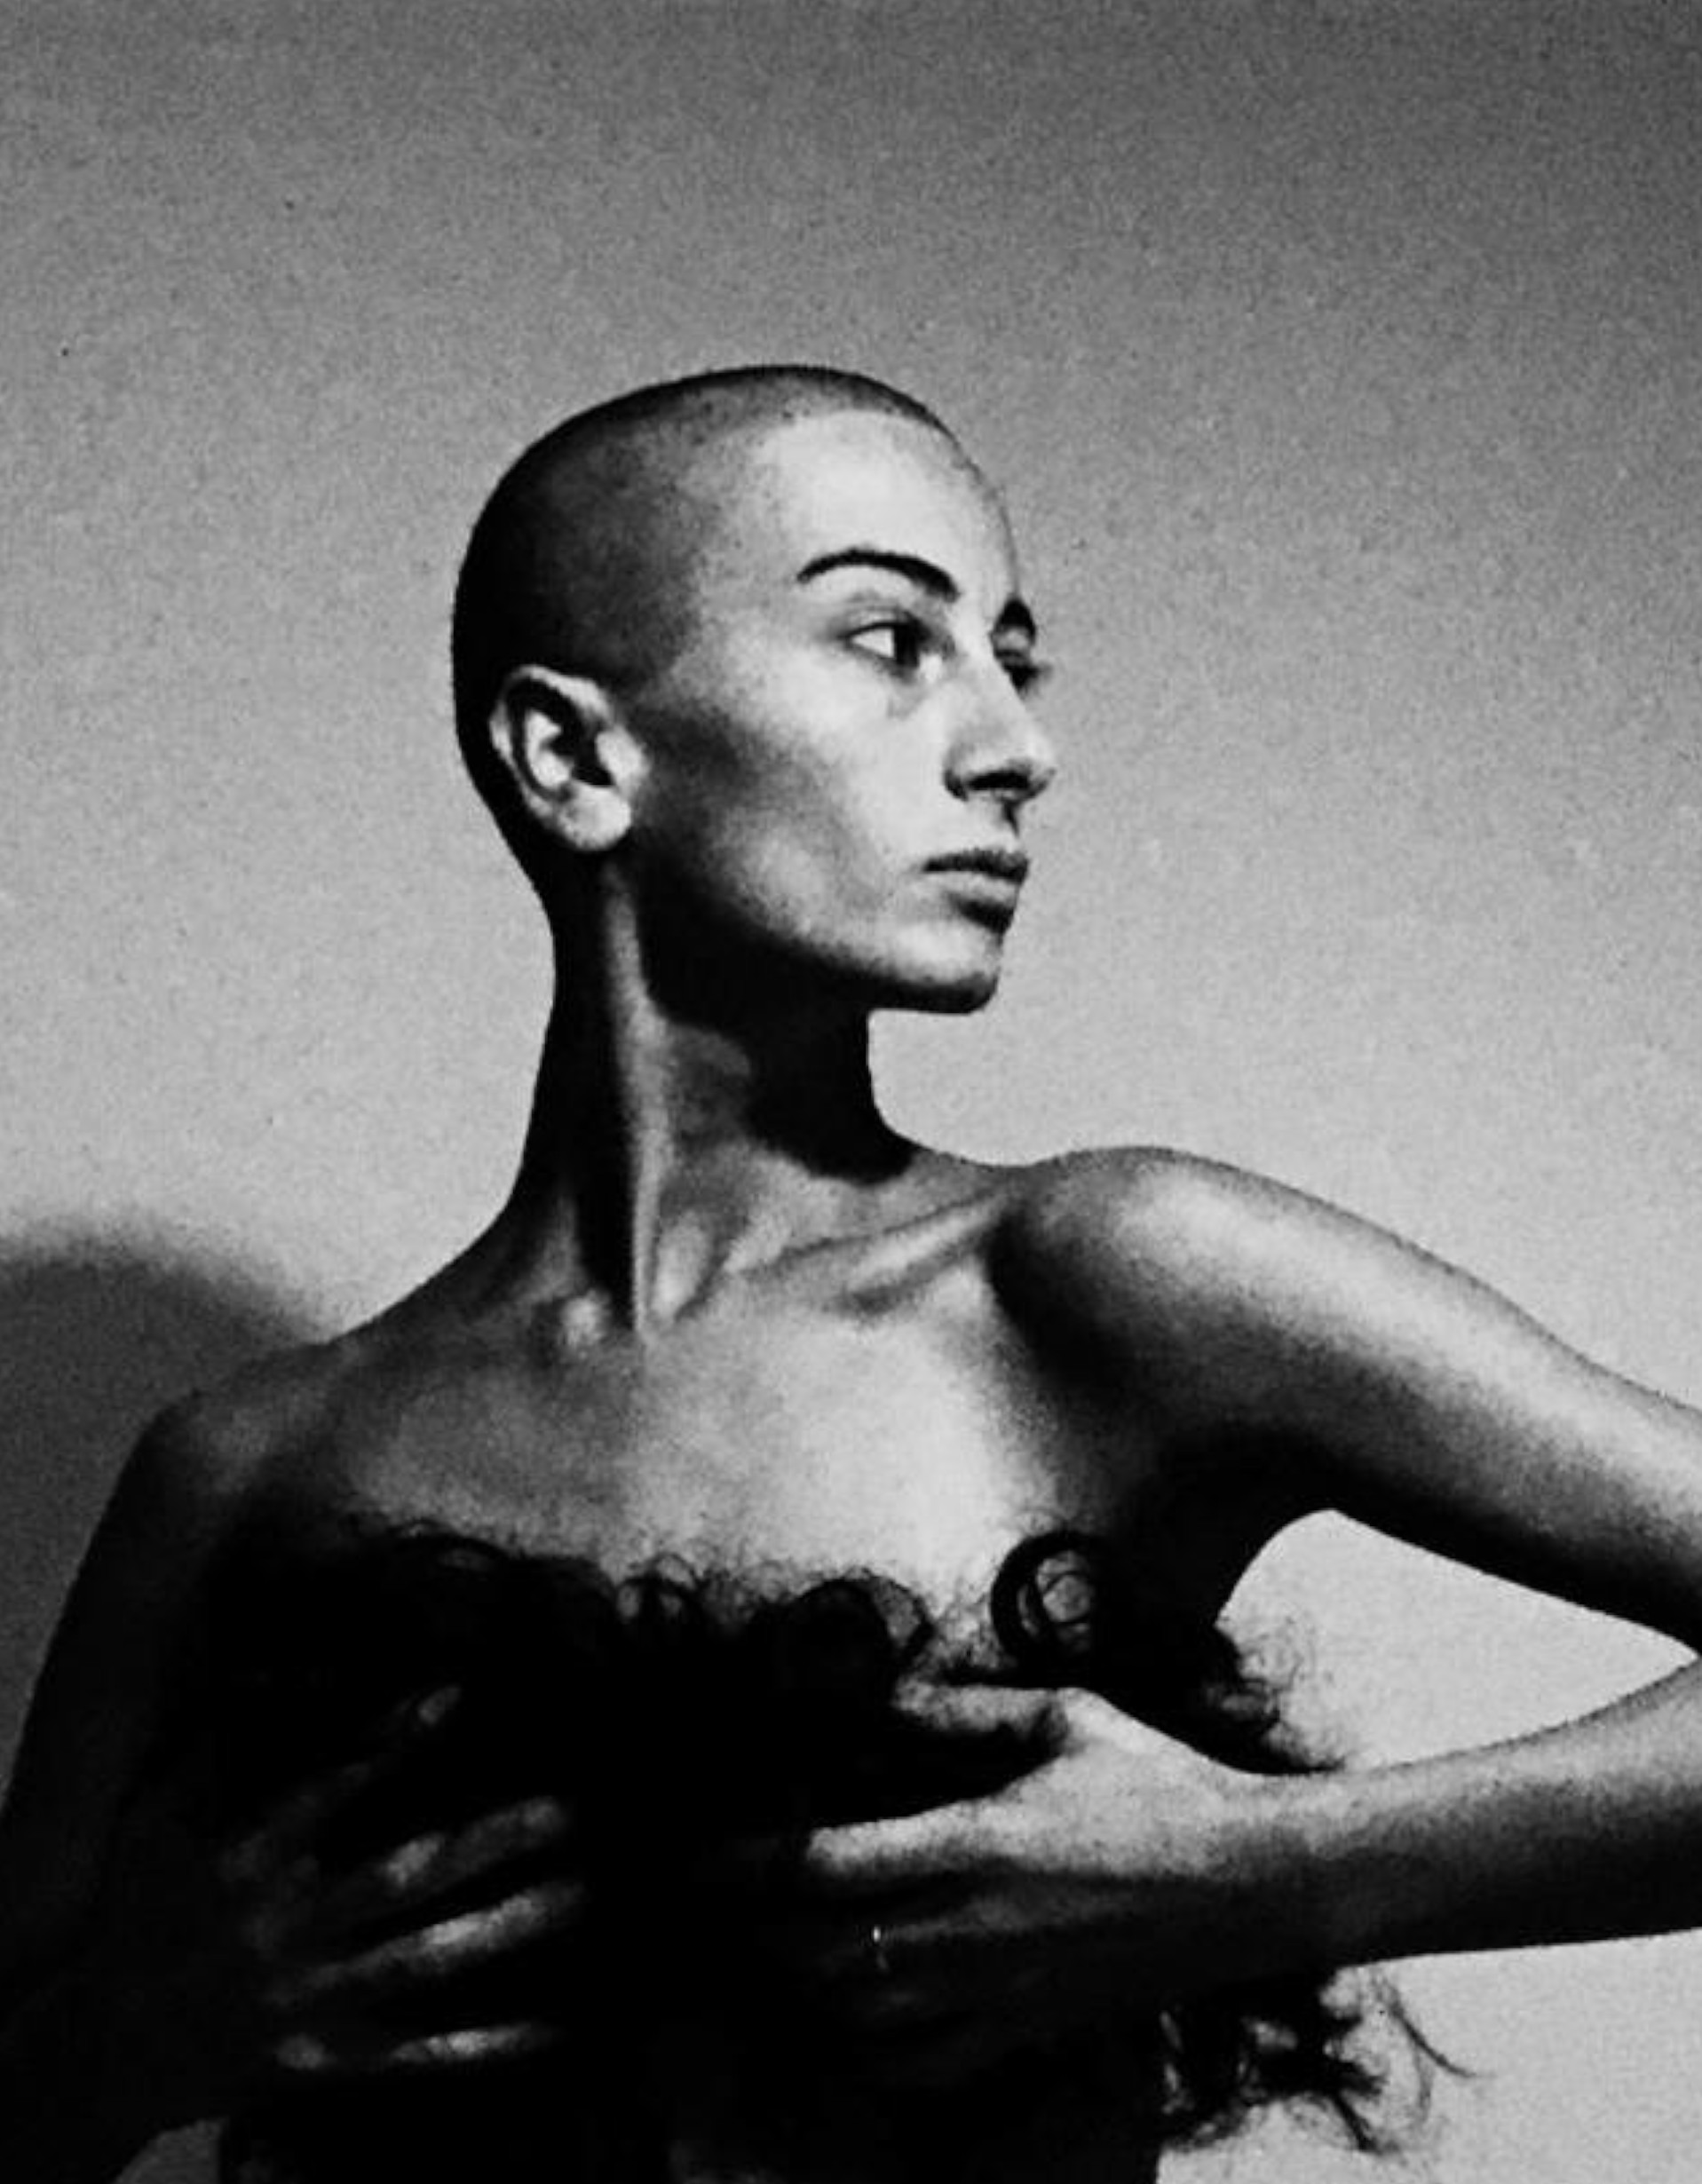
\includegraphics[width=5cm,left]{images/portrait}
    \vspace*{-30pt}
\end{figure}

\MyName{Simon Zimmermann}
\MySlogan{Curriculum Vitae}

\sepspace

%%% ------------------------------------------------------------
\NewPart{Personal details}{}

\PersonalEntry{Birth}{June 5, 1993}
\PersonalEntry{Location}{Düsseldorf, Germany}
\PersonalEntry{Mail}{\url{mail@simonzimmermann.com}}
\PersonalEntry{Github}{\faGithub\space\url{github.com/SimonZimmer}}

%%% ------------------------------------------------------------
\NewPart{Work Experience}{}

\EducationEntry{C / C++ Backend Software Developer}{2022-present}{Dear Reality GmbH, Full-time}{Backend development of digital signal processing algorithms, design of proprietary APIs using C, C++, and Python}
\sepspace
\EducationEntry{C++ Fullstack Software Developer}{2020-present}{Dear Reality GmbH, Full-time}{Full-stack development of real-time desktop audio applications following test-driven development, modern C++, and agile project management principles}
\sepspace
\EducationEntry{Researcher / QA Engineer (Working Student)}{2017-2020}{Dear Reality GmbH, Part-time}{Research and development of digital signal processing prototypes, quality assurance, and test automation development}
\sepspace
\EducationEntry{Room-Acoustics Engineer (Working Student)}{2016-2017}{ISRW-Klapdor, Part-time}{Simulation and design of room-acoustic properties and in-situ acoustic measurements}

%%% ------------------------------------------------------------
\NewPart{Projects}{}
\EducationEntry{dearVR Exoverb}{2022}{Backend Developer}{Developed the DAW-plugin "Exoverb," which uses synthesized reverb impulse responses and additional processing to generate realistic reverberation effects}
\sepspace
\EducationEntry{Team Split Facilitation}{2022}{Backend Developer, DevOps Engineer}{Facilitated the transition from a single-team solution to a frontend/backend split. Extended the technology stack with Conan, Microsoft Azure, Pure Data, and C}
\sepspace
\EducationEntry{dearVR MIX/MONITOR}{2021}{Full Stack Developer}{Developed the DAW-plugins "dearVR MIX" and "dearVR MONITOR," which utilize headphone calibration, room simulation, and binauralization to virtualize professional studio environments. These plugins also simulate multichannel audio playback}
\sepspace

\NewPart{Publication}{}
\EducationEntry{Co-Author}{2021}{Conference Paper, Immersive and 3D Audio: from Architecture to Automotive (I3DA): "Machine Learning-Based Room Classification for Selecting Binaural Room Impulse Responses in Augmented Reality Applications"}
\sepspace

%%% ------------------------------------------------------------
\NewPart{Education}{}

\EducationEntry{M.Sc. Media Informatics}{2018-2020}{University of Applied Sciences Düsseldorf}{Thesis title: 'Scalable Modelling of Room Acoustic Characteristics for AR-devices on the Basis of Visual Information Using Deep Learning' - honors degree.}
\sepspace
\EducationEntry{M.Sc. Music Informatics}{2018}{University of Music Karlsruhe}{Guest Semester}
\sepspace
\EducationEntry{B.Eng. Media Engineering}{2012-2017}{University of Applied Sciences Düsseldorf}{Thesis title: 'A Concept for Implementing Room Acoustic Material Properties in the Context of a 3D-Audio Engine'}
\newpage

%%% ------------------------------------------------------------
\NewPart{Skills}{}

\SkillsEntry{Languages}{German (mother tongue)}
\SkillsEntry{}{English (fluent)}
\sepspace

\SkillsEntry{Technologies}{\textsc{C++17}}
\SkillsEntry{}{CMake}
\SkillsEntry{}{conan}
\SkillsEntry{}{boost}
\SkillsEntry{}{googletest/googlemock}
\SkillsEntry{}{google-benchmark}
\SkillsEntry{}{C99}
\SkillsEntry{}{Python}
\SkillsEntry{}{Pure Data (Pd)}
\SkillsEntry{}{Linux}
\SkillsEntry{}{git}
\SkillsEntry{}{nvim/vim}
\SkillsEntry{}{docker}
\SkillsEntry{}{conan}
\SkillsEntry{}{Azure DevOps}
\SkillsEntry{}{Github Actions}
\SkillsEntry{}{Jenkins}
\SkillsEntry{}{POSIX}
\SkillsEntry{}{MATLAB}
\SkillsEntry{}{\LaTeX}
\SkillsEntry{}{JUCE}
\SkillsEntry{}{pybind11}
\SkillsEntry{}{flask}
\SkillsEntry{}{wagtail}
\sepspace

\SkillsEntry{Other}{Music Production}
\SkillsEntry{}{Modular Synthesizer}
\SkillsEntry{}{Esoteric Programming Lanuages (Orca, TidalCylces)}

\end{document}

